\documentclass[runningheads]{llncs}
\usepackage{graphicx}
\usepackage{amsmath}
\usepackage{ctex}
\newcommand{\upcite}[1]{\textsuperscript{\textsuperscript{\cite{#1}}}}
\begin{document}
\title{航班规划系统设计综述\thanks{Supported by BUAA}}
\author{胡权权}
\institute{北京航空航天大学\ 计算机科学与技术系,北京 100084}
\maketitle
\begin{abstract}
航班规划有多种解决方案,有关图的经典算法大多可以在此方面得到应用,本文重点介绍以往的相关工作,分析对比不同方案的优劣势,综合论述经典算法应用在航班规划方面的常见形式和方法,并尝试基于以往相关工作提出更优的方案。近年来,随着人工智能在诸多方面的广泛应用,其提升航班运行效率也成为可能。 包括航线设计、航班规划、降落规划等,人工智能可以应用在诸多方面。本文结合多篇以往论文和当前人工智能相关研究的进展提出了优化的方法。
\keywords{人工智能  \and 航班规划 \and 效率 \and 优化}
\end{abstract}

%空行是另起一段   
\section{介绍}
在现实世界中,航空公司的航班安排有时无法按照计划进行,造成航班晚点,给航空公司和乘客带来不同程度的损失。航班经常由于恶劣的天气条件、飞机维修、航空临时管制等在不可预知的某天延误或取消,因此航班规划在航空业有着举足轻重的地位,涉及航线安排、航班恢复、大型航空枢纽航班规划等多个方面,对于提升航空网络运行效率、降低航空网络的运输成本、提高乘客满意度等有着重要的意义和作用。对于航空公司而言,合理布局航空网络可以提高公司的竞争力,促进民用航空飞机的生产。航班网络大致可以分为两类:城市到城市(city2city)航班网络、轴辐式(hub-and-spoke)航班网络,后者在欧美大型航空公司更为流行。

历来在航班规划、航班恢复、航线网络设计的研究中,大多有关网络、图的经典算法诸如最短路径算法(Floyd、Dijkstra等)、模拟退火算法、蚁群算法等均有应用。

\section{从乘客角度设计}
航空网络设计问题包括:选择一些城市作为枢纽,按照规则连接不同城市;枢纽之间完全连接,非枢纽城市可以直接连接或者通过枢纽,而且非枢纽城市可以连接一个或多个枢纽。在乘客角度,假设乘客是理智的,以最大化自身利益、最小化自身损失为目标,乘客会选择最便宜的路线旅行,并且考虑时间因素,乘客会优先选择换乘最少的路线。

在(赵天玉\ 等)\upcite{ref_article2}的解决方案中,作者假设国内航空公司的架次最多限制为100架次,跨越距离最大为5500千米,中间转机最多为5次,以深度优先搜索作为基本算法;同时考虑旅游经济,要求算法能通过路径删除和节点删除产生多重解,在多重解中寻找最优的航班规划;考虑经济成本,以里程为最小代价函数,求出最优解(最经济的航班规划情况)。以乘客为出发点,从多重解中寻找最优解来进行航班规划,然而盲目的深度优先搜索或者广度预先搜索的效率并不高,如果算法采用启发式搜索将能提高一定的效率。启发式信息可以是某种极大值或极小值:转机次数最少、里程最短,采用最小成本法的思想进行启发式搜索会有更好的效果,因此作者采用的就是以深度优先搜索作为基本算法,以路 径删除和结点删除方法并用产生多重解,以最小成本 法为优化条件,产生最优解。产生多重解有路径删除法和结点删除法两种方法,路径删除法从数据库中删除所有形成当前这个解的结点,然后再试求另外的解; 结点删除方法只要简单地删除当前求解路径中的最后一个结点,并且继续搜索即可。不足之处:在搜索到结果之后仍会运行计算出与其他结点(机场)的连接情况,降低效率,此模型未考虑航班时长,换乘时长。

\section{从航空公司角度设计}
大多数航班网络都是轴辐式(hub-and-spoke)的结构,Mark John Hall 等人对比了欧洲两家航空公司的数据\upcite{ref_article15},发现枢纽机场的航班和乘客远远多于普通机场,建立了对航空运输系统(ATS)的深入理解。由于经典算法是NP-hard问题,不能有效的解决问题,结合Floyd最短路径的蚁群算法\upcite{ref_article10}也有应用,这种方案重点关注轴辐式(hub-and-spoke)航班网络。针对这种航班网络设计的相关研究早就在进行,Campbell(1994)就这个问题建立0-1整数规划模型\upcite{ref_article20},1996年他又提出了一种称为Greedy Interchange 的算法来完善这个问题\upcite{ref_article21}。Skorin-Kapov提出一个有效的0-1混合整数规划\upcite{ref_article22},并利用LP松弛算法得到了最优解。

然而航空网络设计问题是一个NP完全问题,经典算法无法有效解决,所以启发式算法的研究越来越多,例如Zhong Yuan-xiang 和 Chen Zheng-fang 提出的一种基于tuba搜索的模拟退火算法\upcite{ref_article23},BAI Ming-guo提出的基于tuba搜索和最短路径的启发式算法\upcite{ref_article24},实验结果表明这些算法是有效的。在Yi QIN等2009年的工作中\upcite{ref_article10},作者建立了没有具体轮毂数量的数学模型,为了避免算法陷入局部解,使算法易于用代码实现,作者结合了蚁群算法,以蚂蚁在网络中的可见程度作为启发式信息,引导蚂蚁选择下一个城市,选择合理的城市作为枢纽,然后确定网络的连接方式,以最小化运输成本和枢纽建设成本为目标函数,此种方案适用于大型航空公司网络设计。2010年,Yi Qin 等人又提出了一种具有人类学习能力的蚁群算法(HACA),针对运输成本和航空流量的不确定性,采用鲁棒优化方法建立了新的数学模型\upcite{ref_article16},通过假设枢纽机场已被选定并且容量有限,进而确定中心机场与其他机场的连接来在不确定需求和运输成本的条件下确定机场间的最优连接,HACA算法经验证可以避免过早陷入局部解,有效地提高了解的多样性。

随着空中交通量的增长,很多国内航空公司开始关注航班网络的优化,国内航空公司大多参照发达国家航空的运营网络模式---轴辐式(hub-and-spoke)网络进行优化。Jing Xiong 等人通过对航空机队规划的研究\upcite{ref_article14},以航空公司运营路径网络利润最大化、成本最小化模型建立目标函数,对中国国内民航企业融入全球市场提出参考。WU Wei-wei 等人应用集队理论(Set pair Theory)\upcite{ref_article25},考虑市场需求、航线运营成本和机场容量,研究了对于航空公司如何选择开发新的航线,从而优化航班网络结构、提高公司经济收益和竞争力。针对如何建设城市中心辐射网络,ZHANG Yan 等人采用鲁棒优化方法对航班规划过程进行优化,引入Dijkstra改进初始解和领域结构\upcite{ref_article12},计算结果表明方案在航空公司航班优化有良好的效果,对国内航空公司网络优化有着一定的指导意义。ZHANG Yan等人之后又提出了用于智能航班规划的改进禁忌搜索算法\upcite{ref_article11},引入专门的Floyd最短路径方法来改善初始解和邻域结构,对于航空公司网络而言,最短路径通常意味着路线上的成本最小化,可以通过找到每对节点之间的最短路径来解决连接状态的问题,并且可以通过重复找到最佳和第二最佳解决方案。作者仅选择了北京、上海、广州和西安四个城市作为中心城市,未来工作将深入研究区域一级作为中心机场的应用。

航空公司航班机队分配问题在理论上属于整数规划,针对国内航线的单中心辐射网络的特点,大多数经典算法(如分支限界法)导致性能不佳,Yu Wang等人首先基于单轴辐式(hub-and-spoke)航班网络作预处理,减少航班规划问题的规模,通过直接路径的随机分解,使用模拟算法求解航班机队分配\upcite{ref_article13},方案稳定效率较高,这种方案基于单中心辐射航班网络,作者未来的研究将支持运行多中心分支的轴辐式网络。

%插图
% \begin{figure}[ht]
% \centering
% 
\includegraphics[scale=0.1]{404.jpg}
% \caption{this is a figure demo}
% \label{fig1}
% \end{figure}

\section{兼顾乘客和航空公司的设计}
航空公司花费大量时间、精力、人力、物力、财力等资源在航班规划上,最大限度的减少公司损失同时提高乘客满意度、提高公司商誉。

然而航空公司总会面对不可预见的意外,例如恶劣天气、机场拥堵、机械故障等,如果找到成本最小化、时间最小化的航班规划使航空公司从混乱中恢复至关重要。LU Rong-qin 等人的工作以最小化航空公司和乘客损失为目标函数,考虑了本场航班离港延误成本、外场航班离港延误成本以及外场航班进港延误成本三个要素,建立了0-1整数规划模型\upcite{ref_article5}。作者根据干线、VIP乘客和大飞机等因素来确定航班优先级,引入 s 作为大飞机系数。规划模型如下:

\begin{multline*}
   min\ Z = \sum_{i_b}C_{d,i_b}P_{i_b}\left[\sum_{t_n}x_{i_b,t_n}t_n-t_{i_b,0}\right]+ \\ \sum_{i_w}C_{d,i_w}P_{i_w}\left[\sum_{t_n}x_{i_w,t_n}t_n-t_{i_w,0}\right]+\left[\sum_{t_{en}}x_{i_w,t_{en}}t_{en}-t_{i_w,en0}\right] \\
\end{multline*}  

公式中第 1 部分表示本场航班离港延误成本,第 2 部分表示外场航班离港延误成本,第 3 部分表示外场航班进港延误成本$i_b$为本场航班集合;$C_{d,i_b}$为本场航班的单位时间延误系数;$P_{i_b}$为本场航班延误系数;$x_{i_b,t_n}$为0-1变量,表示本场第 i 个航班在 $t_n$ 时刻出港时为 1 ,否则为0;其余变量对应外场航班参数。考虑的情况比较周全,然而航空约束条件不止作者涉及的限制条件,还有诸如航空管制、机组人员调度安排、航班资源约束等,在多参数、复杂约束情况下还需要更合理高效的解决方案。

\begin{figure}[ht]
\centering
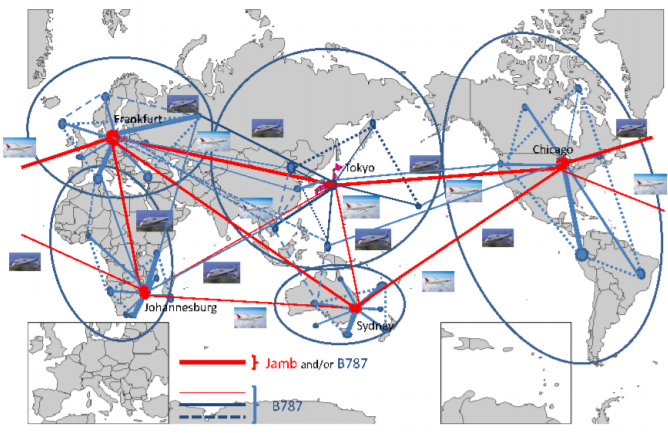
\includegraphics[scale=0.8]{nstar.png}
\caption{不久的未来航空多星网络示意图}
\label{fig1}
\end{figure}

在北美乃至全球航空网络中,都有同样的一个重要特征,即更多航线倾向于连接到重要的结点(航空枢纽或者大型都市),这在英文中被称为"preferential attachment",即航空枢纽的附加优惠。Hidefumi Sawai 认为这种航班网络还有提高效率的空间\upcite{ref_article9},他受到蚁群优化算法(ACO)的启发,设计了一种小世界(SW)网络,利用ACO自组织小世界网络,进而形成多星网络(n-star),其航线的平均长度较短。空客A380机型的停产也在某种程度上应验了作者的观点,未来航班规划都在往多航线、多中小机型方面发展。这种n个星形结点组成的架构能让乘客有更多路线选择、减少乘客换乘次数,而且作为星形结点的重要城市均完全连接形成集团,节省里程和巡航距离、降低航空公司的运营成本,Hidefumi Sawai 小世界(SW)模型预测未来的全球航空网络示意图(见图\ref{fig1})。

关于航班恢复规划类似的工作还有很多,Stojković等人\upcite{ref_article26}开发了一种网络模型,可以最大限度地减少乘客的总延误,并使用分支定界启发式求得问题最优解,在理论上有很好的效果,但是难以应用到现实中。Xiuli等人\upcite{ref_article27}提出了一种结合GRASP和禁忌搜索的混合启发式算法。Dozić等人\upcite{ref_article28}开发了一种启发式算法,它可以交换部分轮转数据并返回一系列较优的解。Eggenberg等人\upcite{ref_article29}提出了一个约束特定的恢复网络模型,它们通过列生成解决方案。Rosenberger等人\upcite{ref_article30}将飞机恢复问题建模为集合打包问题,并使用飞机选择启发式来确定飞机的子集以减小整数规划问题规模的大小。Jarrah等人\upcite{ref_article31}使用最小成本网络模型,一个延迟模型和一个消除模型,并实现了一种算法,该算法反复解决最短路径问题,以确定必要的流量。SINCLAIR等人\upcite{ref_article4}提出基于列生成的后优化启发式算法来规划航班和乘客的恢复,采用混合整数线性规划模型,并采用LNS启发式算法降低问题规模。Meilong Le等人\upcite{ref_article8}综合论述了恢复航班的规划问题的研究,对比了不同工作的进展。

\section{从其他方面入手的设计}
在航线、机场日益增多的情况下,航班时刻优化的相关研究随之增多。然而相关的研究多数往往仅考虑了航空公司的经济效益或者空中交通流量管理,为此胡明华\ 等人提出一种改进的匈牙利算法\upcite{ref_article1},对两者综合考虑,基于以往的航班数据,以增加虚拟航班的形式将航班规划转化为指派问题,迭代寻找最优解。在对单个机场航班规划的设计上表现良好,作者将进一步针对机场网络进行航班规划算法的研究和改进。

大多数航班延误都是由于机场过于繁忙造成拥堵和运力不平衡导致的,Jacquillat等人\upcite{ref_article6}通过缓解机场拥堵方面进行航班规划,借助航班调度、优化航班时刻表等多种方法提出综合规划办法,开发了一种原始的迭代算法,集成随机排队机场模型、容量利用动态规划模型和整数规划模型,在JFK机场的大量计算表明模型的效果。Pyrgiotis等人\upcite{ref_article7}等人研究了诸如临时航班管制等一些不可避免地原因造成行程限制地影响,提出对航班规划的指导。

David W. Hutchison等人\upcite{ref_article17}通过仿真模拟航班延误来促进航班管理和规划,由于航班管理系统非常复杂,作者使用了SIMMOD模拟程序(ATAC Corporation 1995)在4个机场的航班网络上模拟336个航班的流量,通过加入扰动和惩罚函数来解决航班规划这种高维约束优化问题。

针对枢纽机场的选址问题也对航班规划有着重要意义,Banu Soylu等人\upcite{ref_article18}提出了一种精确的启发式帕累托边界查找算法来确定新的枢纽机场的选址,第一个目标为最小化网络的总运输成本,而第二个目标为最小化两站式旅行,以提高客户满意度,这也许会受到航空公司多条运输路线的负面影响。尽管使用枢纽降低了网络运营成本,但成本效益高的枢纽网络并不意味着乘客体验舒适或旅行时间最短。乘客更喜欢乘坐停站较少的航班,但是这样会增加网络的运营成本。如何权衡找到其帕累托边界是作者集中的焦点,作者提出可变领域搜索启发式算法来逼近大型航班网络的帕累托边界。

Seyed Sina Mohria等人\upcite{ref_article19}另辟蹊径,他们从机场容量包络曲线入手设计轴辐式(hub-and-spoke)航班网络,提出了一种新的实用的航空公司轮毂容量决策模型,对一些小规模的伊朗航空公司网络进行了精确求解,针对大型航空公司网络提出了具有移动自适应的大领域搜索算法。

\section{总结}
本文简要回顾了近些年航班规划领域的相关研究进展,根据航班规划设计考虑的对象对文献进行了简单分类论述,有些模型部分算法有着或多或少的相同,求解方法大致有启发式、数学规划、混合法三类。航班规划是一种高维约束问题,这种NP-hard问题以整数规划求解效果不甚理想,而启发式算法的相关研究众多。几类算法各有优劣:

\begin{table}
\centering
\begin{tabular}{lp{6cm}p{3cm}p{3cm}}
\hline
算法 &  举例 & 优缺点\\
\hline
启发式算法 &  {\bfseries Stojković等人\upcite{ref_article26}的分支限界启发式算法} & 不会陷入局部最优解,但是响应慢\\
整数规划算法 &  {\bfseries Campbell等人\upcite{ref_article20}的0-1整数规划模型} & 易于求解,难以应对NP-hard问题\\
混合算法 & {\bfseries Rosenberger等人\upcite{ref_article30}采用启发式算法降低整数规划问题规模} & 结合响应快、求解合理的优点,算法复杂\\
% 3rd-level heading & {\bfseries Run-in Heading in Bold.} Text follows & 10 point, bold\\
% 4th-level heading & {\itshape Lowest Level Heading.} Text follows & 10 point, italic\\
\hline
\end{tabular}
\caption{启发式、整数规划、混合法三类算法对比.}\label{tab1}
\end{table}


% \noindent Displayed equations are centered and set on a separate
% line.
% \begin{equation}
% x + y = z
% \end{equation}
% Please try to avoid rasterized images for line-art diagrams and
% schemas. Whenever possible, use vector graphics instead (see
% Fig.~\ref{fig2}).

% \begin{figure}
% 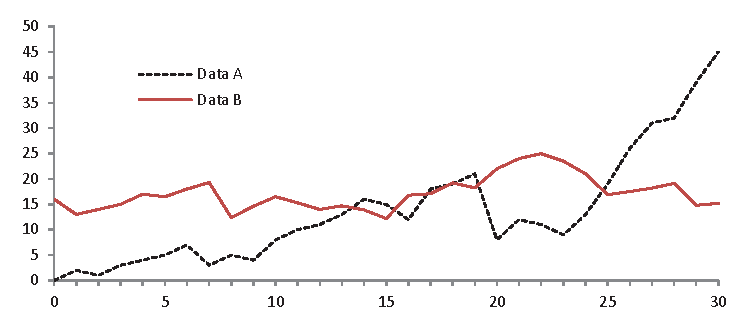
\includegraphics[width=\textwidth]{fig1.eps}
% \caption{A figure caption is always placed below the illustration.
% Please note that short captions are centered, while long ones are
% justified by the macro package automatically.} \label{fig2}
% \end{figure}

% \begin{theorem}
% This is a sample theorem. The run-in heading is set in bold, while
% the following text appears in italics. Definitions, lemmas,
% propositions, and corollaries are styled the same way.
% \end{theorem}
%
% the environments 'definition', 'lemma', 'proposition', 'corollary',
% 'remark', and 'example' are defined in the LLNCS documentclass as well.
%
% \begin{proof}
% Proofs, examples, and remarks have the initial word in italics,
% while the following text appears in normal font.
% \end{proof}
% For citations of references, we prefer the use of square brackets
% and consecutive numbers. Citations using labels or the author/year
% convention are also acceptable. The following bibliography provides
% a sample reference list with entries for journal
% articles~\upcite{ref_article1}, an LNCS chapter~\upcite{ref_lncs1}, a
% book~\upcite{ref_book1}, proceedings without editors~\upcite{ref_proc1},
% and a homepage~\upcite{ref_url1}. Multiple citations are grouped
% \upcite{ref_article1,ref_lncs1,ref_book1},
% \upcite{ref_article1,ref_book1,ref_proc1,ref_url1}.
%
% ---- Bibliography ----
%
% BibTeX users should specify bibliography style 'splncs04'.
% References will then be sorted and formatted in the correct style.
%
% \bibliographystyle{splncs04}
% \bibliography{mybibliography}
%
\begin{thebibliography}{8}
% \bibitem{ref_article1}
% Author, F.: Article title. Journal \textbf{2}(5), 99--110 (2016)

\bibitem{ref_article1}
胡明华, 裔田园, 任禹蒙. 基于改进匈牙利算法的机场航班时刻优化研究[J/OL]. 2019, 36(8). [2018-04-24]. 

\bibitem{ref_article2}
赵天玉: 基于人工智能的飞机航班信息查询系统的设计[J]. 计算机与现代化, 2005, (08):27-29.

\bibitem{ref_article3}
HU Y Z, LIAO H, ZHANG S, et al. Multiple Objective Solution Approaches for Aircraft Rerouting Under the Disruption of Multi-aircraft[J]. Expert Systems with Applications, 2017, 83:283-299.

\bibitem{ref_article4}
SINCLAIR K, CORDEAU J F, LAPORTEG G. A Column Generation Post- Optimization Heuristic for the Integrated Aircraft and Passenger Recovery Problem[J]. Computers and Operations Research, 2016, 65:42-52.

\bibitem{ref_article5}
陆荣琴, 赵小梅, 毕军, 张俊. 基于航班综合影响因素的延误航班重排问题的整数规划模型[J]. 交通运输研究, 2017, 3(03):36-42.

\bibitem{ref_article6}
Jacquillat A, Odoni A R. An Integrated scheduling and operations approach to airport congestion mitigation. [J]. Operations Research, 2017, 63 (6):1390-1410. 

\bibitem{ref_article7}
Pyrgiotis N, Odoni A. On the impact of scheduling limits: a case study at newark liberty international airport [J]. Transportation Science, 2016, 50:150112072345006. 

\bibitem{ref_article8}
Meilong Le, Congcong Wu, Chenxu Zhan and Lihong Sun, "Airline recovery optimization research: 30 years' march of mathematical programming—A classification and literature review," Proceedings 2011 International Conference on Transportation, Mechanical, and Electrical Engineering (TMEE), Changchun, 2011, pp. 113-117.

\bibitem{ref_article9}
H. Sawai, "Reorganizing a new generation airline network based on an Ant-Colony Optimization-inspired Small-World network," 2012 IEEE Congress on Evolutionary Computation, Brisbane, QLD, 2012, pp. 1-8.

\bibitem{ref_article10}
Y. Qin, J. Zhu and Wei Zhang, "Airline network design with variable hub number," 2009 2nd International Conference on Power Electronics and Intelligent Transportation System (PEITS), Shenzhen, 2009, pp. 1-4.

\bibitem{ref_article11}
Y. Zhang and J. Zhang, "An improved tabu search algorithm application to intelligent airline network optimization," 2009 2nd International Conference on Power Electronics and Intelligent Transportation System (PEITS), Shenzhen, 2009, pp. 312-315.

\bibitem{ref_article12}
Y. Zhang and J. Zhang, "Dijkstra's algorithm based robust optimization to airline network planning," 2010 International Conference on Mechanic Automation and Control Engineering, Wuhan, 2010, pp. 2783-2786.

\bibitem{ref_article13}
Y. Wang and H. Sun, "Application of Simulated Annealing Algorithm in Airline Fleet Assignment Problem," 2010 International Conference on Intelligent System Design and Engineering Application, Changsha, 2010, pp. 364-367.

\bibitem{ref_article14}
J. Xiong, X. Zhang and Q. Du, "Research on an optimization model of airline fleet planning," 2016 IEEE Information Technology, Networking, Electronic and Automation Control Conference, Chongqing, 2016, pp. 469-472.

\bibitem{ref_article15}
M. J. Hall, R. Ravindranath, P. Bermell-Garcia and A. Johansson, "Route networks within the air transport system: A comparative study of two European low-cost airlines using network metrics," 2016 Annual IEEE Systems Conference (SysCon), Orlando, FL, 2016, pp. 1-6.

\bibitem{ref_article16}
Y. Qin, J. Zhu and Wei Zhang, "The robust optimization of the capacitated hub and spoke airline network design base on ant colony algorithms," 2010 International Conference on Intelligent Computing and Integrated Systems, Guilin, 2010, pp. 601-604.

\bibitem{ref_article17}
David W. Hutchison and Stacy D. Hill. 2001. Airline and airport applications: simulation optimization of airline delay with constraints. In Proceedings of the 33nd conference on Winter simulation (WSC '01). IEEE Computer Society, Washington, DC, USA, 1017-1022.

\bibitem{ref_article18}
Banu Soylu,Hatice Katip. A multiobjective hub-airport location problem for an airline network design[J]. European Journal of Operational Research,2019,277(2).

\bibitem{ref_article19}
Seyed Sina Mohri, Hossein Karimi, Ali Abdi Kordani, Mahdi Nasrollahi,Airline hub-and-spoke network design based on airport capacity envelope curve: A practical view Computers and Industrial Engineering,Volume 125,2018.

\bibitem{ref_article20}
Campbell J F. Integer programming formulations ofdiscrete hub location problems(1]. European Journal of Operational Research, 1994,72 : 387405.

\bibitem{ref_article21}
Campbell J F. Hub location and the p - hub median problem[J]. Operations Research, 1996,44(6):923 - 935.

\bibitem{ref_article22}
Skorin - Kapov D, Skonrin - Kapov J, O'kelly M. Tight linear programming relaxations ofuncapacitated p - hub median problem (1]. European Journal ofOperational Research, 1996,94 : 582 - 593.

\bibitem{ref_article23}
ZHONG Yuan-xiang, CHEN Zheng-fang. A heuristic research on multiallocation p-median problem.[A]. The first session of the Taiwan Society of Operations Research Symposium 2004 Symposium on Technology and Management [C]. Taibei, 2004, 75 - 81.

\bibitem{ref_article24}
BAI Ming-guo,ZHU Jin-fu,XU Jin. A heuristic algorithm on p-hub airline network design problem(1]. Operation Research and Management, 2007, 16(4): 64 - 68. 

\bibitem{ref_article25}
W. Wu and J. Zhu, "Research on Airline Route Scheme Optimization Model," 2009 WRI World Congress on Software Engineering, Xiamen, 2009, pp. 391-396.

\bibitem{ref_article26}
Stojković M, Soumis F, Desrosiers J, Solomon MM. An optimization model for a real-time flight scheduling problem. Transp Res Part A 2002;36:779–88. 

\bibitem{ref_article27}
Xiuli Z, Yanchi G. An improved GRASP for irregular flight recovery. In: 2012 International Conference on System science and engineering (ICSSE); 2012. 

\bibitem{ref_article28}
Dozić S,KalićM,BabićO.Heuristicapproachtotheairlinescheduledisturbances problem: single fleet case. Proced—Soc Behav Sci 2012;54:1232–41. 

\bibitem{ref_article29}
Eggenberg N, Salani M, Bierlaire M. Constraint-specific recovery network for solving airline recovery problems. Comput Oper Res 2010;37:1014–26. 

\bibitem{ref_article30}
Rosenberger JM, Johnson EL, Nemhauser GL. Rerouting aircraft for airline recovery. Transp Sci 2003;37:408–21.

\bibitem{ref_article31}
Jarrah AIZ, Yudeci G. A decision support framework for airline cancellations and delays. Transp Sci 1993;27:266–80. 

\bibitem{ref_article32}
DUAN Hai-bin. Principle and Application of ant colony algorithm[M]. Beijing : Science press, 2005.

\bibitem{ref_article33}
Guo Chonghui, Yue Xiaohui, "An Improved Tabu Search Algorithm and application to global progressively optimization" [1], Operation and Management, 2007,16 (4) :6211.

\bibitem{ref_article34}

\bibitem{ref_article35}

\bibitem{ref_article36}

\bibitem{ref_article37}

\bibitem{ref_article38}

\bibitem{ref_article39}

\bibitem{ref_article40}

\bibitem{ref_article41}

\bibitem{ref_article42}

\bibitem{ref_article43}

\bibitem{ref_article44}

\bibitem{ref_article45}

\bibitem{ref_article46}




% \bibitem{ref_lncs1}
% Author, F., Author, S.: Title of a proceedings paper. In: Editor,
% F., Editor, S. (eds.) CONFERENCE 2016, LNCS, vol. 9999, pp. 1--13.
% Springer, Heidelberg (2016). \doi{10.10007/1234567890}

% \bibitem{ref_book1}
% Author, F., Author, S., Author, T.: Book title. 2nd edn. Publisher,
% Location (1999)

% \bibitem{ref_proc1}
% Author, A.-B.: Contribution title. In: 9th International Proceedings
% on Proceedings, pp. 1--2. Publisher, Location (2010)

% \bibitem{ref_url1}
% LNCS Homepage, \url{http://www.springer.com/lncs}. Last accessed 4
% Oct 2017
\end{thebibliography}
\end{document}
